\graphicspath{{figures/dynamic/}}

\chapter{考虑龙卷风平移的动态响应分析}

第\ref{chapter:static}章忽略了龙卷风平移运动的影响,
分别在\SI{0}{\degree}、\SI{45}{\degree}和\SI{90}{\degree}工况下进行静力非线性分析。
本章考虑龙卷风平移运动的影响,假定其移动轨迹后计算输电塔结构各节点荷载时程,
进行动力时程分析,分析其动态响应。

\section{动态龙卷风模型}

根据第\ref{sec:tower-fea}建立整体坐标系,如图\ref{fig:tower-tornado-cs}所示。
龙卷风相应于输电塔结构做平移运动的示意图见图\ref{fig:tornado-path}\todo{replot}所示。
\begin{figure}[!htpb]
	\centering
	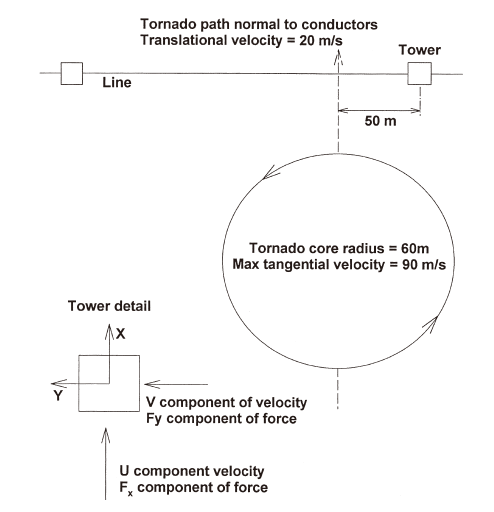
\includegraphics[width=0.6\textwidth]{tornado-path.png}
	\caption{龙卷风相应于输电塔做平移运动的示意图}
	\label{fig:tornado-path}
\end{figure}

\subsection{龙卷风路径}

假定龙卷风核心在地面上做匀速直线运动,描述其路径的关键参数为核心初始位置和运动速度。

为了使得初始时刻输电塔结构所受龙卷风荷载较小,需要将龙卷风核心初始位置设置在距离输电塔较远的地方。
若初始时刻龙卷风核心距离输电塔很近,结构会受到量值很大的突加荷载的影响,与实际情况不符。
初始位置在整体坐标系中的位置记为$\left(x^T_{0},y^T_{0}\right)$。

关于龙卷风的平移速度在第\ref{sec:tornado-cha}节已有介绍,
我国《三十万千瓦压水堆核电厂安全重要土建结构抗龙卷风设计规定》中A类龙卷风平移速度为\SI{22.4}{m/s},
文献\cite{savory2001modelling}\cite{hamada2011behaviour}中选用龙卷风平移速度为\SI{20.0}{m/s},
二者差别较小,本文为计算简便选用$v^T=\SI{20.0}{m/s}$。
确定龙卷风路径还需龙卷风平移速度的方向,设平移速度相对于输电线、即$X$轴正向的夹角为$\theta^T$。

综上,龙卷风运动轨迹$\left(x^T(t),y^T(t)\right)$可表示为:
\begin{equation}
	\begin{cases}
		x^T(t) = x^T_0 + \left(v^T\cos{\theta^T}\right)t \\
		y^T(t) = y^T_0 + \left(v^T\sin{\theta^T}\right)t 
	\end{cases}
\end{equation}
龙卷风的平移运动引起了龙卷风核心相对输电塔位置$\left(x^T(t),y^T(t)\right)$随时间变化,
进而使得输电塔受到了随龙卷风位置变化的荷载时程,需进行动力时程分析计算结构响应。

本文假设龙卷风风场结构不随时间变化(实际中龙卷风会随其运动衰减,本文忽略这一现象),
即采用第\ref{sec:full-tornado}中模拟的足尺龙卷风风场作为任一时刻动态龙卷风的风场。

\section{动态龙卷风风速及荷载时程}

在任意时刻$t$,利用第\ref{sec:static-code}节中规范方法施加该时刻的龙卷风荷载。
由于第\ref{sec:static-code}节已编制了计算龙卷风荷载并施加到输电塔结构的APDL程序,
在动力分析中,改变龙卷风核心相应于输电塔中心的极坐标$(R,\theta)$(见第\ref{sec:d-polor}节),
调用龙卷风荷载施加子程序,即可完成动态荷载施加过程。

输电塔结构在龙卷风时变荷载作用下的动态响应由动力时程分析计算。
时间步长选用\SI{0.10}{s}。
并进行时间步长的敏感性分析,发现当时间步长减小为\SI{0.05}{s}时结构动态响应差别较小。
这说明\SI{0.10}{s}的时间步长是足够精确的。

\subsection{典型龙卷风运动工况}

龙卷风平移运动的两种典型工况见图\ref{fig:dynamic-case1}和图\ref{fig:dynamic-case2}。
图\ref{fig:dynamic-case1}中龙卷风运动路径平行于输电线,下文简称为龙卷风平行运动工况;
图\ref{fig:dynamic-case2}中龙卷风运动路径垂直于输电线,下文简称为龙卷风垂直运动工况。

\begin{figure}[!htpb]
    \centering
    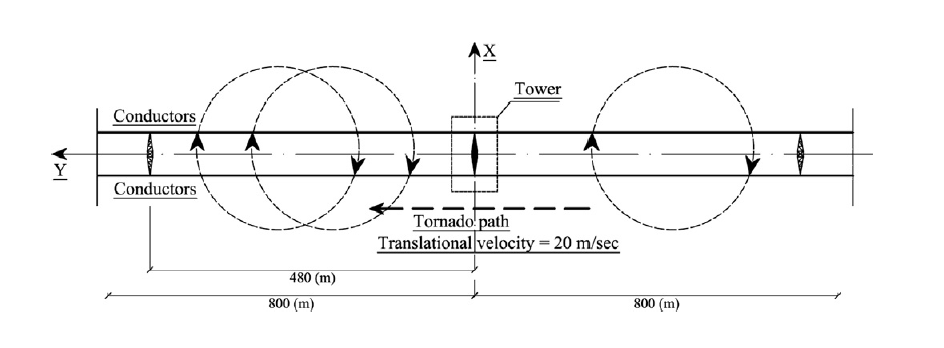
\includegraphics[width=0.8\textwidth]{dynamic-case1.png}
    \caption{龙卷风平行运动工况}
    \label{fig:dynamic-case1}
\end{figure}
\begin{figure}[!htpb]
    \centering
    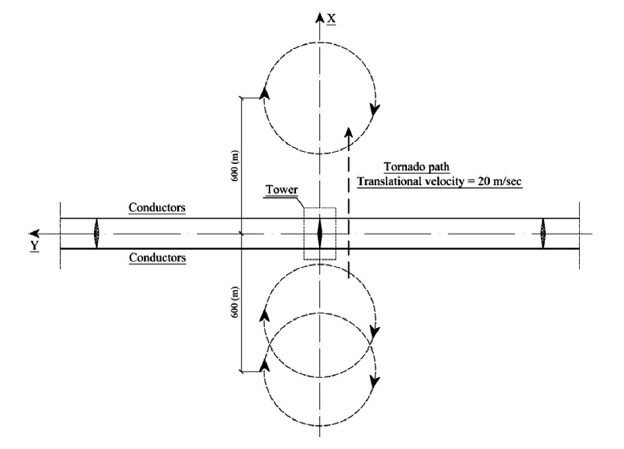
\includegraphics[width=0.8\textwidth]{dynamic-case2.png}
    \caption{龙卷风垂直运动工况}
    \label{fig:dynamic-case2}
\end{figure}

平行运动工况(图\ref{fig:dynamic-case1})中,
龙卷风核心初始位置选为$x_0^T=\SI{1500}{m}$,$y_0^T=\SI{120}{m}$;
平移速度$v^T=\SI{20.0}{m/s}$,$\theta^T=\pi$。
满足初始时刻龙卷风距离输电塔较远,龙卷风荷载较小,
且在运动过程二者距离取得龙卷风核心半径$r_c=\SI{120}{m}$,受到龙卷风荷载较大。

类似选取垂直运动工况(图\ref{fig:dynamic-case2})的参数,
龙卷风核心初始位置选为$x_0^T=\SI{120}{m}$,$y_0^T=\SI{1500}{m}$;
平移速度$v^T=\SI{20.0}{m/s}$,$\theta^T=-\frac{1}{2}\pi$。

\subsection{动态龙卷风风速时程}

\subsection{动态龙卷风荷载时程}

\section{输电塔结构动态时程分析}
